\documentclass{article}
\usepackage{graphicx,hyperref,enumitem}
\usepackage[super]{nth}

\topmargin=-.25in
\setlength{\textwidth}{6.75in}
\setlength{\textheight}{8.8in}
\setlength{\oddsidemargin}{0in}
\setlength{\evensidemargin}{0in}
\setlength{\parskip}{2ex}
\setlength{\parindent}{0in}

\newcommand{\Rin}[1]{\textbf{$>$ {#1}}}
\newcommand{\Rcom}[1]{\hspace{1cm} \#{#1}}
\newcommand{\Rout}[1]{\texttt{{#1}}}

\begin{document}
\pagestyle{myheadings}\markright{
CU Boulder \hspace{0.5in} MATH 2510 - Introduction to Statistics }

\begin{center}
\textbf{\underbar{Project 2 - Due Tuesday, May 1}}
\end{center}

The focus of this project is to expose you to some of the features in R, a programming language and environment that can be used in statistics. In particular, in this project you will compute various statistics for data sets, generate random sets of data to analyze, and compute probabilities. Previous experience in programming (R or other languages) is not required for this project, although you may find the R environment easier to adapt to, if you have some.

Note that R Studio is available in computer labs campus-wide. If you do not have a computer with R Studio installed, you can get this for free at \url{http://www.rstudio.com/}. Also note that you must have an R distribution installed on your computer as well, which you can also get for free at \url{https://cran.r-project.org/}.

The project is due by class on Tuesday, May 1. There are two components: A worksheet which you will complete using your results from R-workspace, and an R-workspace file containing all required components. The worksheet is to be handed in class. The R-workspace will need to be submitted via the D2L Dropbox. The workspace file you submit will be loaded into an R-session by your instructor and graded based on accurate values of objects you are instructed to define in the project. So, make certain that you use {\em EXACTLY} the object names stated in the instructions. Also note, object names are \textbf{case-sensitive!}

You must work in groups of 2 or 3, handing in one worksheet and submitting one R-workspace for the group.  On Thursday, April 12, you will be asked to specify your group members. A single Dropbox in D2L will be created for your group. You will need to upload your R-workspace to D2L by classtime on Tuesday, May 1. You will hand in the worksheet in class on that date, as well.

There is information about saving your workspace in the Tutorial and in one of the Screencasts available for this project. This step is crucial to complete correctly to make sure that you are submitting ALL of your work.

There is a brief introduction and Tutorial available for this project in the Project 2 Content folder in D2L. A set of screencasts showing an active R-environment is also available there. The screencasts available are
	\begin{itemize}
	\item Intro to R including help, basic object assignment, and data editing %help.start(), c, data.entry
	\item Saving and loading a workspace
	\item Using some of the basic statistics commands %mean, median, sd, weighted.mean
	\item Creating random samples and histograms %sample and hist
%	\item Importing data %read.csv
	\item Using basic probability functions %pnorm, qnorm, dbinom, pbinom
	\end{itemize}

There are also many resources online for help and tutorials on the tasks required of you in this project.

\newpage 
For those of you who have no experience with R, here is a screenshot of what the R-Studio interface looks like on a Mac. \\
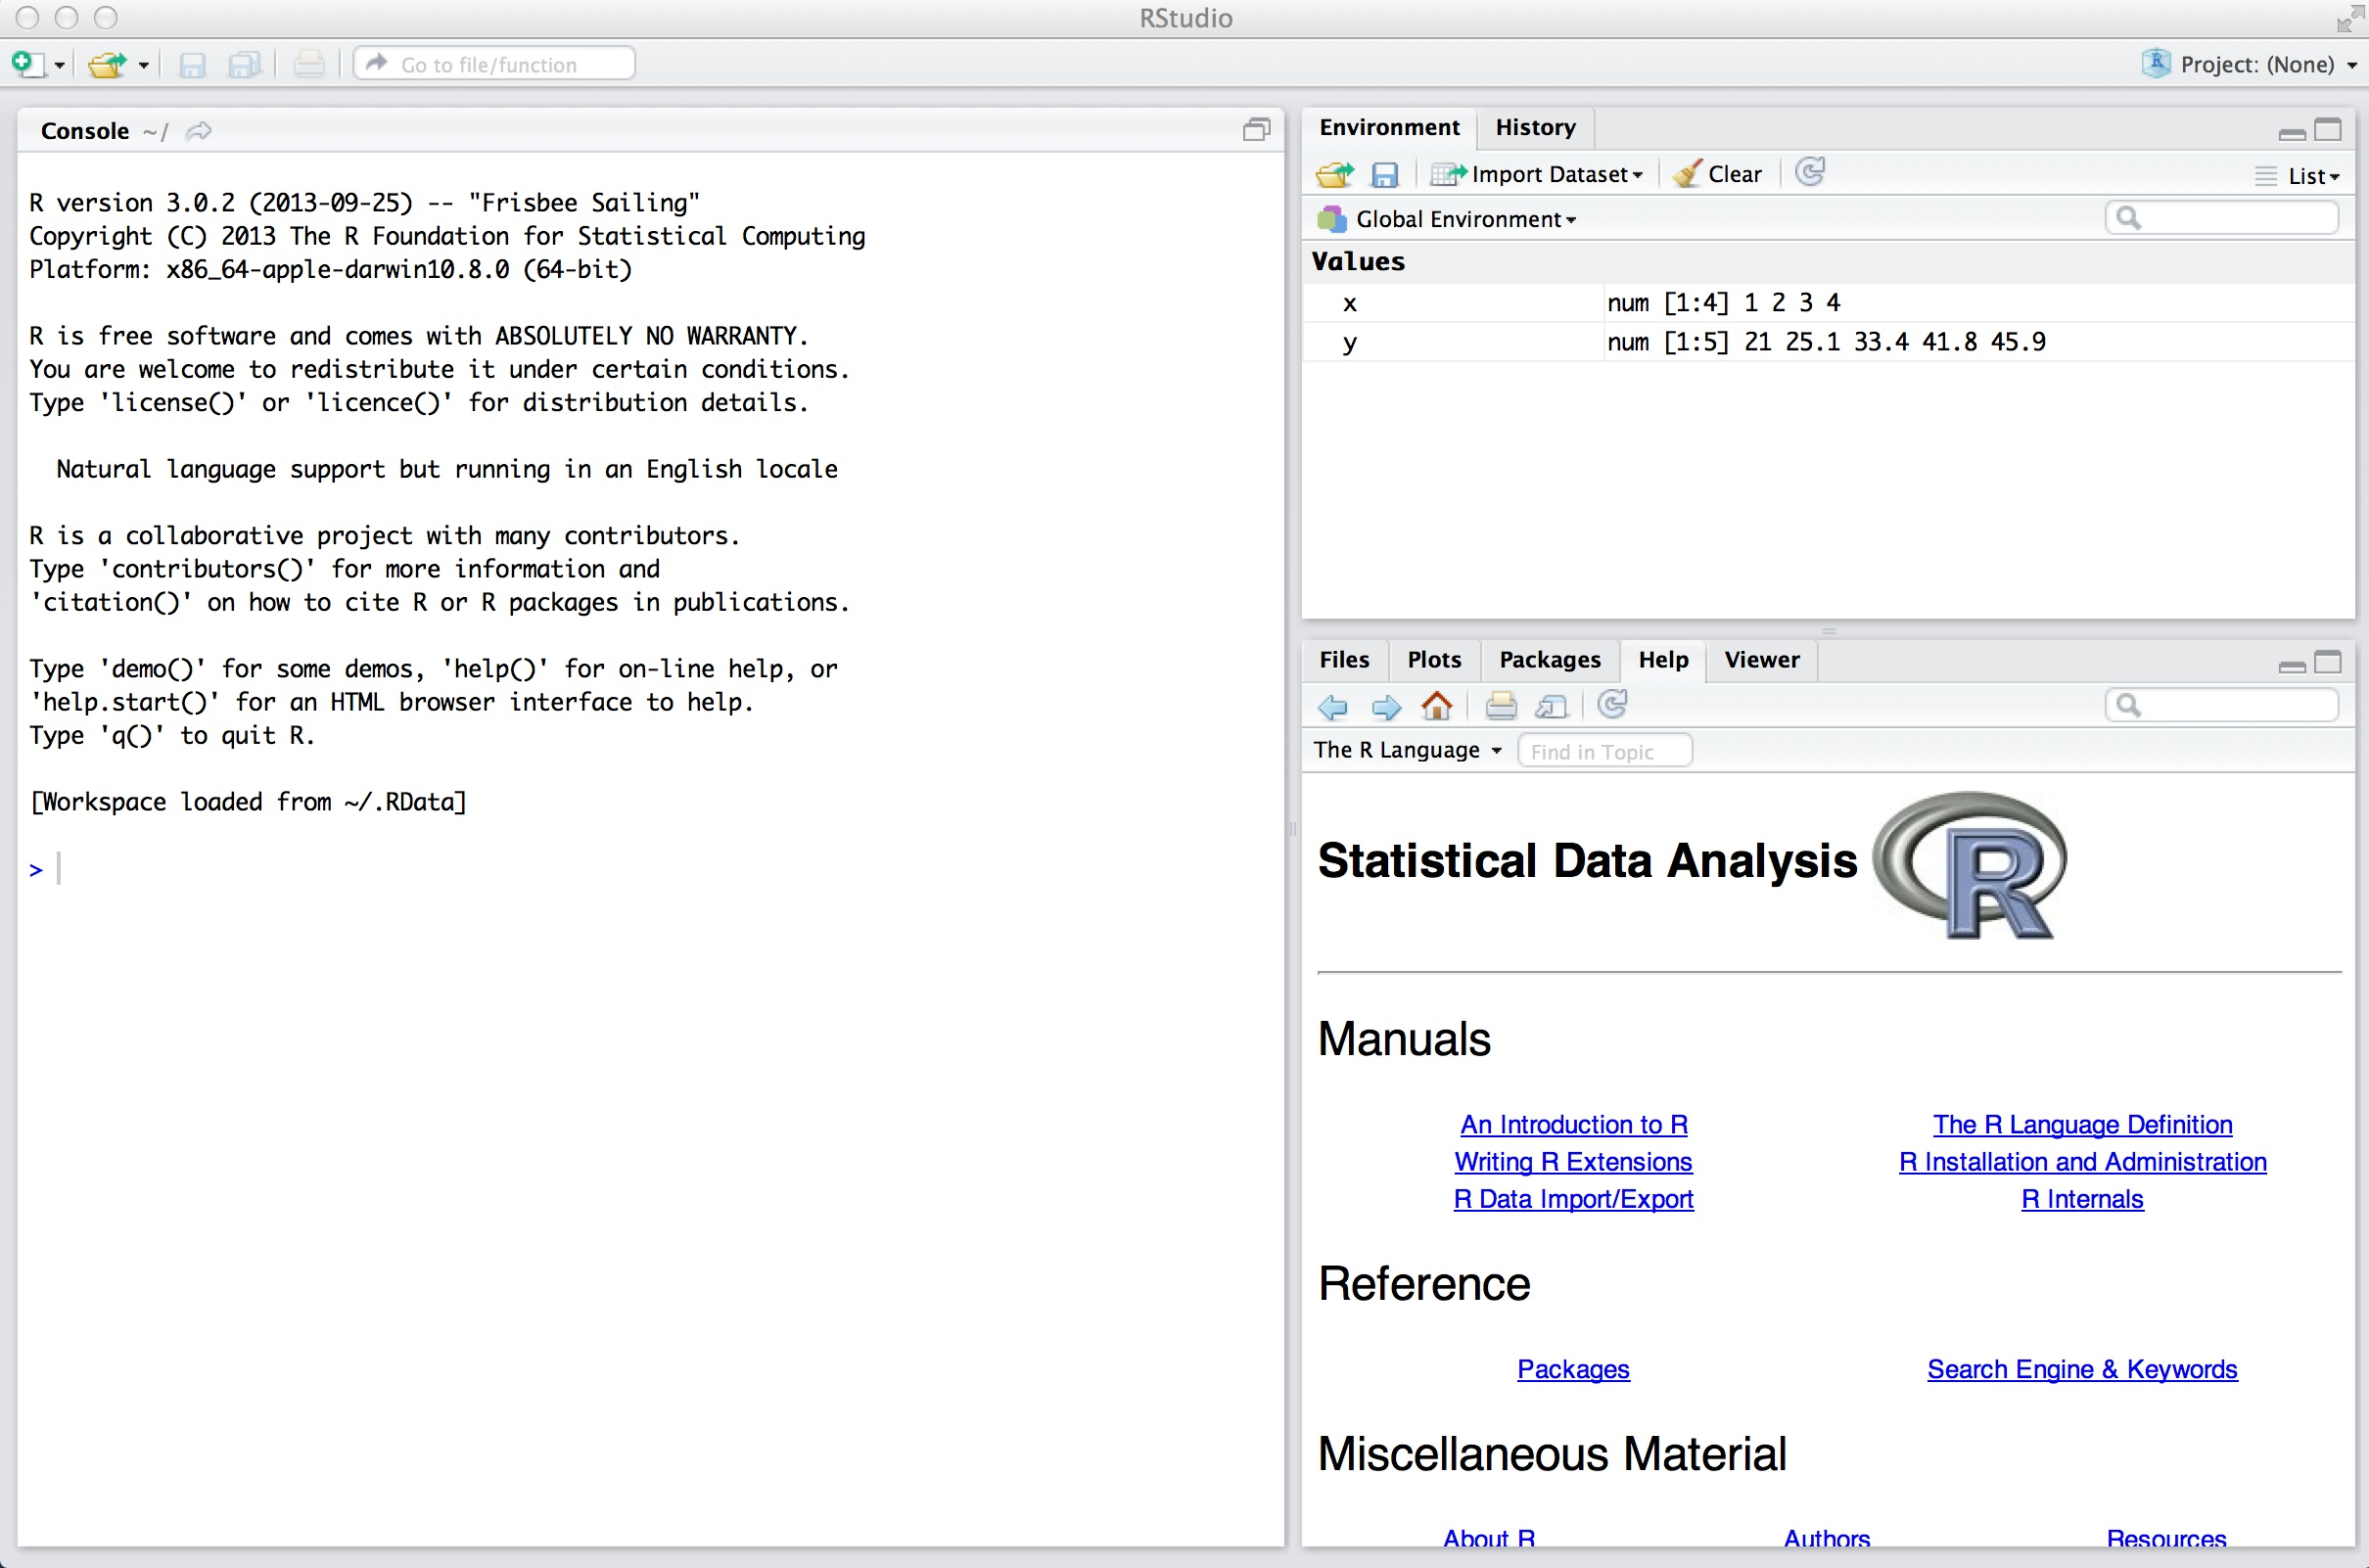
\includegraphics[scale=0.3]{RStudio.jpg}

\newpage
%Project Instructions

\begin{enumerate}

% Object list: Name
\item To begin, create an object called `Name' that is a list containing the names of all group members. You will need to use quotation marks around each name to identify the input as text.

% #1 Object list : x1, x1ave, x1med, x1sd, x1new, x1len
\item This problem asks you to manually create a list of data values called `x1' (that's $x$ and {\em one}) and perform some basic computations and manipulations with that list. Make sure that you are using the object names {\em EXACTLY} as stated here and that the objects are saved to the workspace file that you submit.
	\begin{enumerate}
	\item Create an object named `x1' that is a list consisting of the seven data values \{1,3,5,6,6,7,9\}.
	\item Use the \texttt{mean} function to compute the mean of `x1' and assign that value to the object `x1ave'.
	\item Use the \texttt{median} function to compute the median of `x1' and assign that value to the object `x1med'.
	\item Use the \texttt{sd} function to compute the standard deviation of `x1' and assign that value to the object `x1sd'.
	\item Add the five data values \{1,2,4,7,9\} to the end of `x1' and assign that new list to the object `x1new'.
	\item Use the \texttt{length} function to compute the number of data values in `x1' and assign that value to the object `x1len'.
	\end{enumerate}
	
%#2 Object list: x2, x2term, x2ave, x2sd, x2new, x2newterm
\item This problem asks you to create a list (called `x2') of random data values and perform some basic analysis of the list. Again, make sure that you are using the object names {\em EXACTLY} as stated here and that the objects are saved to the workspace file that you submit.
	\begin{enumerate}
	\item Use the \texttt{sample} function to create a random list of 300 integers between $1$ and $10$ (inclusive). Assign this list to the object `x2'.
	\item Determine the value of the \nth{202} integer in this list and assign that value to the object `x2term'.
	\item Assign the mean value of this list of numbers to the object `x2ave'.
	\item Assign the standard deviation value of this list of numbers to the object `x2sd'.
	\item Add 1700 more random integer values between $1$ and $10$ (inclusive) to the end of `x2' and assign that new list of 2000 random integers to the object `x2new'.
	\item Determine the value of the \nth{1250} integer in this new list and assign that value to the object `x2newterm'.
	\end{enumerate}
	
%#3 Object list: x3, x3ave, x3newadj
%\item This problem asks you to import data from an external csv file which holds a frequency table into an object (called `x3'), edit the data, and compute the mean. And, yes, make sure that you are using the object names {\em EXACTLY} as stated here and that the objects are saved to the workspace file that you submit.
%	\begin{enumerate}
%	\item Use the \texttt{read.csv} function to import the two column data set from the file ExamScores.csv (available in D2L in the Project 2 folder) and assign it to the object `x3'.
%	\item Use the \texttt{weighted.mean} function to compute the mean exam score and assign that value to the object `x3ave'. Note: Using myarray[[i]] calls the $i$th column of `myarray', similar to how mylist[i] calls the $i$th item of `mylist'.
%	\item Once entered, you realize that there are four scores of 100 that were not recorded in the csv. Use the \texttt{data.entry} function to update `x3' to add the four missing scores of 100 to the data file. Alternatively, you can edit the .csv file elsewhere (such as Excel) and re-import the file. \emph{\textbf{WARNING: } The data.entry function causes R to crash on some Apple computers.}
%	\item Use the \texttt{weighted.mean} function to compute the mean exam score of the adjusted `x3' and assign that value to the object `x3aveadj'.
%	\end{enumerate}

%#4 Object list: x4, x4ave, x4sd, samp45, samp45ave, x4distr, x4distrterm, x4distr2, x4distr2ave, x4distr2sd, x4lower, x4upper
\item This problem asks you to create a random distribution that is not normal (called `x4'), analyze a random sample from this distribution, and then to illustrate the Central Limit Theorem by creating a distribution of $\bar{x}$ values. Oh yeah, you should really make sure that you are using the object names {\em EXACTLY} as stated here and that the objects are saved in the workspace file that you submit.
	\begin{enumerate}
	\item Assign to the object `x4' a random distribution of 8000 values using the following R-command. \\
	\Rin{x4 = c(rpois(8000, c(10, 40)))}.
	\item Assign the mean value of the distribution `x4' to the object `x4ave'.
	\item Assign the standard deviation of the distribution `x4' to the object `x4sd'.
	\item Use the \texttt{hist} function to create a histogram of the `x4' data distribution. (Just use the system defaults for all parameters.) Print this histogram and attach it to your worksheet to turn in. \\
	(As advertised, this distribution should not look like a normal distribution...does it?)
	\item Use the \texttt{sample} function to generate a random sample of 60 values (without replacement) from `x4'. Assign this data set to the object `samp60'.
%	\item Determine the value of the $32^{nd}$ value in `samp45'. Assign this value to the object `samp45term'.
	\item Assign the mean of the sample `samp60' to the object `samp60ave'.
	\item In order to illustrate the Central Limit Theorem, we must have a sampling distribution consisting of a large number of sample means. Enter the following lines of code to generate 300 samples each of size 60, compute the mean of each sample, and assign that list of 200 sample means to the object `x4distr'. \\
	\Rin{x4distr = c()} \Rcom{Creates a new empty list named `x4distr'} \\
	\Rin{for(i in 1:300)\{samp = sample(x4, 60, replace=F); x4distr = c(x4distr, mean(samp))\}}
	\item Determine the sample mean for the \nth{250} sample you just selected. That is, determine the \nth{250} item on the `x4distr' list and assign that value to the object `x4distrterm'.
	\item Although 300 is a large number of samples, programming makes it very easy to increase the number of samples and even alter the sample size. Create a sampling distribution consisting of 30,000 sample means where each sample has size 120 and assign that list to the object `x4distr2'.
	\item Create a histogram of the `x4distr2' data distribution. (Just use the system defaults for all parameters.) Print this histogram and attach it to your worksheet to turn in. \\
	(Hint: According to the Central Limit Theorem, what shape should the sampling distribution have? Does it?)
	\item Assign the mean and standard deviation of the sampling distribution `x4distr2' to the objects `x4distr2ave' and `x4distr2sd', respectively.
	
  \item Use the code below to determine a list of 95\% confidence intervals for the population mean based on each of the samples that made 'x4distr2'. Specifically, `x4lower' will be a list of the lower bounds and `x4upper' will be a list of the upper bounds. \\
  To determine the actual interval for the \nth{810} sample (for example), you would use the \nth{810} item from the `x4lower' list and the \nth{810} item from the `x4upper' list and the \nth{810} item from the `x4distr2' list should be the midpoint of those two values.\\
  \Rin{x4lower = x4distr2 + qnorm(.025)*x4sd/sqrt(120)} \\
  \Rin{x4upper = x4distr2 + qnorm(.975)*x4sd/sqrt(120)}
	\end{enumerate}

%#5 Object List: x5a, x5b, x5c, x5d, x5e
\item This problem will ask you to use appropriate functions of R to answer probability questions similar to the ones we have be doing in class. (Hmmm...I wonder if these objects should be saved and named exactly as indicated??)
	\begin{enumerate}
	\item The amount of ketchup dispensed from a machine at a local convenience store is normally distributed with a mean of $1.20$ ounces and a standard deviation of $0.087$ ounce. Use the \texttt{pnorm} function to determine the probability that the machine dispenses more than 1 ounce for a giving serving? Assign that value to the object `x5a'.
	\item The scores on the SAT are normally distributed. The mean SAT score during a certain year was 995 with a standard deviation of 175. Use the \texttt{qnorm} function to determine the cutoff score for the $\nth{88}$ percentile. Assign that value to the object `x5b'.
	\item Use the \texttt{dbinom} function to compute the probability of a (fair) coin landing heads {\em exactly} $92$ times in $153$ flips of the coin. Assign that value to the object `x5c'.
	\item A student is taking a 50-question multiple-choice quiz, each with 5 answer choices (only one of which is correct). Use the \texttt{pbinom} function to determine the probability that the student answers no more than 15 questions correct if that student randomly guesses the answer to every question on the quiz. Assign that value to the object `x5d'.
	\item A six-sided die is biased so that the probability of rolling a 4 on the single roll of the die is only 10\%. Use the following while loop to determine the minimum number to times the die would need to be rolled so that the probability of rolling a total of fifty or more 4's is at least 90\%. Assign that minimum number of rolls to the object `x5e'. (HINT: What variable is counting the number of rolls?) \\
	\Rin{n=50} \Rcom{We can start with $n=50$ rolls since we are looking for at least 50 successes.} \\
	\Rin{while(1-pbinom(49, n, .10) $<$ .90)\{n = n+1\}}
	\end{enumerate}

\item Now make sure to save your workspace and upload it to the D2L Dropbox by the due date. You can use the \texttt{ls()} function to list all the objects in your workspace and check that all 30 required objects are there. Extra objects are fine as they will simply be ignored. But all of the required items on the rubric must be named EXACTLY as listed (including case) or the grader will ignore them too. \\
\{Name, x1, x1ave, x1med, x1sd, x1new, x1len, x2, x2term, x2ave, x2sd, x2new, x2newterm, x4, x4ave, x4sd, samp60, samp60ave, x4distr, x4distrterm, x4distr2, x4distr2ave, x4distr2sd, x4lower, x4upper, x5a, x5b, x5c, x5d, x5e\}

\end{enumerate}	

\newpage
%Worksheet
\begin{center}
\textbf{\underbar{Project 2 Worksheet - Due Tuesday, May 1}}
\end{center}

NAME 1:{\underbar{\hspace{2in}}} \hfill NAME 2:{\underbar{\hspace{2in}} 

\bigskip

NAME 3:{\underbar{\hspace{2in}}

\begin{enumerate}

\item Suppose ``Y1" is an object where \Rin{length(Y1)} yields \Rout{[1] 5} and \Rin{mean(Y1)} yields \Rout{[1] 4.4}. Suppose ``Y2" is an object where \Rin{length(Y2)} yields \Rout{[1] 10} and \Rin{mean(Y2)} yields \Rout{[1] 7.3}. \\
If we assign \Rin{Y3 = c(Y1, 5, Y2)}, then write the output for
	\begin{enumerate}
	\item \Rin{length(Y3)}
	\vspace{0.25cm}
	\item \Rin{mean(Y3)}
	\vspace{0.25cm}
	\end{enumerate}
	
\item Attach the frequency histograms for `x4' and `x4distr2'.
\vspace{0.5cm}

\item Of the 30,000 samples taken from `x4', what is the mean of the \nth{810} sample? What is the confidence interval based on the \nth{810} sample? What is the population mean of `x4'? Does that specific interval actually contain the population mean of `x4'?
\vspace{2cm}

\item For the 30,000 confidence intervals for the samples from `x4', about how many would you expect to contain the mean of `x4'? Explain.
How many of the intervals actually contain the mean? What code did you type in to get this? \\
HINT: You might find the following code, that counts the number times the mean is less than the upper bound, helpful to get you started on determining the relevant line of code:\\
  \Rin{sum(x4ave $<$ x4upper)}
  \vfill

\item According to the Central Limit Theorem, what should the (theoretical) value of $\mu_{\bar{x}}$ equal for {\em your} specific x4distr2 sampling distribution? Write an equation in terms of the object names used in this project. How do your empirical results match the theoretical results of the theorem? That is, how does the actual value of the $\mu_{\bar{x}}$ value for your x4distr2 compare to the theoretical value that it should be?
  \vfill
  
\newpage

\item According to the Central Limit Theorem,what should the (theoretical) value of $\sigma_{\bar{x}}$ equal for {\em your} specific x4distr2 sampling distribution? Write an equation in terms of the object names used in this project. How do your empirical results match the theoretical results of the theorem? That is, how does the actual value of the $\sigma_{\bar{x}}$ value for your x4distr2 compare to the theoretical value that it should be?
\vfill

\item Determine which of the four probability functions \{\texttt{dbinom, pbinom, pnorm, qnorm}\} is most appropriate to compute the answer to the following question. Then write the exact R-code that should be entered to compute that answer, as well as the answer. \\
{\em Denver Nuggets player Gary Harris has a free throw percentage of 79.1\% (we can say that the probability that Gary makes a single free throw is 79.1\%). If Gary attempts 30 free throws, what is the probability that he makes at most 20 of them? Assume each free throw is independent of all others.}
\vfill

\item Using the \texttt{while}-loop provided in the quota problem in 5e as a guide, write the exact R-code that should be entered to solve the following problem, as well as the answer.  \\
{\em The probability that a skeet shooter can hit 41 or more targets in 60 total shots is $0.451$. Find the probability of this shooter hitting the target when he shoots at a single target. Provide an answer accurate to 4 decimal places.}\\
So, you know the cumulative probability $P(r \geq 41) = 0.451$. But, now determine the probability of success on a single attempt using a \texttt{while}-loop.
 \vfill
\end{enumerate}

\end{document}

